%BEGIN_FOLD
%----------------------------------------------------------------------------------------
%	PACKAGES AND OTHER DOCUMENT CONFIGURATIONS
%----------------------------------------------------------------------------------------

\documentclass[12pt, a4paper, twocolumn, fullpage]{article}

\usepackage{color}
\usepackage{graphicx}
\usepackage{amssymb}
\usepackage{amsthm}
\usepackage{lipsum}
%\usepackage[round]{natbib} TODO in future
\usepackage{titlesec}
\titleformat*{\section}{\Large\bfseries}
\titleformat*{\subsection}{\large\bfseries}

\usepackage{amsmath,amsfonts,amssymb,amsthm,epsfig,epstopdf,titling,url,array}


\theoremstyle{plain}
\newtheorem{thm}{Theorem}[section]
\newtheorem{lem}[thm]{Lemma}
\newtheorem{prop}[thm]{Proposition}
\newtheorem*{cor}{Corollary}

\theoremstyle{definition}
\newtheorem{defn}{Definition}[section]
\newtheorem{conj}{Conjecture}[section]
\newtheorem{exmp}{Example}[section]

\theoremstyle{remark}
\newtheorem*{rem}{Remark}
\newtheorem*{note}{Note}

%---------
%	ARTICLE INFORMATION
%----------------
\title{Topological Classification of SCOPe}
\author{Yechan Hong, Jan Segert, and Jianlin Cheng
\and University of Missouri, Columbia}
\date{\today}
%END_FOLD
\begin{document}
\maketitle

% ====================================
\section*{Abstract}
% ====================================

\textbf{Motivation:} SCOPe 2.07 is a database of 276,231 protein domains that have been partitioned into varying folds according to their shape and function. Since a protein's fold reveals valuable information about it's shape and function, it is important to find a mapping between protein's and it's fold. There are existing techniques to map a protein's sequence into a fold \cite{deepsf} but none to map a protein's shape into a fold. We focus on the topological features of a protein to map it into a fold. We introduce several new techniques that accomplish this.
\\
\textbf{Results:} We develop a 2D-convolutional neural network to classify any protein structure into one of 1232 folds. 
We extract two classes of input features for each protein's carbon alpha backbone: distance matrix and the persistent homology barcodes. Due to restrictions in our computing resources, we make sample every other point in the carbon alpha chain. We find that it does not lead to significant loss in accuracy.
Using the distance matrix, we achieve an accuracy of 86\% on the entire dataset.

We extract significant topological simplices of the protein by using persistent homology. We format the persistent homology data into various input features: persistence images \cite{persistenceImages}, simplex distance map, and simplex grouping.  With persistence images of 100x100 resolution, we achieve an accuracy of 62\% on SCOP 1.55. With simplex distance maps of 100x100 resolution, we achieve an accuracy of 70\%. With simplex groupings, we achieve an accuracy of :TODO\%.
	
%	We also combine the different classes of input features to achieve an accuracy of :TODO\%. An analysis on the network is performed to qualitatively describe the features the network is using to accurately classify the proteins.

% ====================================
\section{Introduction}
% ====================================
	Add introduction in literature and background information here. Future work to be added here. Discussion of topological data analysis will also be added here.

% ====================================
\section{Material}
%====================================

%----------------------
\subsection{Datasets}
%----------------------

The SCOP database is a database of proteins organized into hierarchical classes based on their shape and function. There are 4 levels of the hierarchy (top down): Class, Folds, Superfamily, Family. We will be primarily concerned with the Fold.

Two different versions of the dataset were used, SCOP 1.55 and SCOPe 2.07. SCOP 1.55 is a smaller dataset which is a subset of SCOPe 2.07, a larger and more recent dataset. SCOP 1.55 [Ref: Biblio] and SCOPe 2.07 [Ref: Biblio] were downloaded from the Berkeley repository as tar files and unpacked. For each of the datasets, index files [Ref:Biblo] are provided.

\subsubsection{Small Dataset SCOPe1.55}

SCOP 1.55 is a dataset of 31,474 proteins that have been organized into 7 Classes, 605 Folds, 947 Superfamilies, and 1557 Families. The dataset was released and updated till 2001. This dataset is a subset of the SCOPe 2.07 dataset.

\begin{figure}
	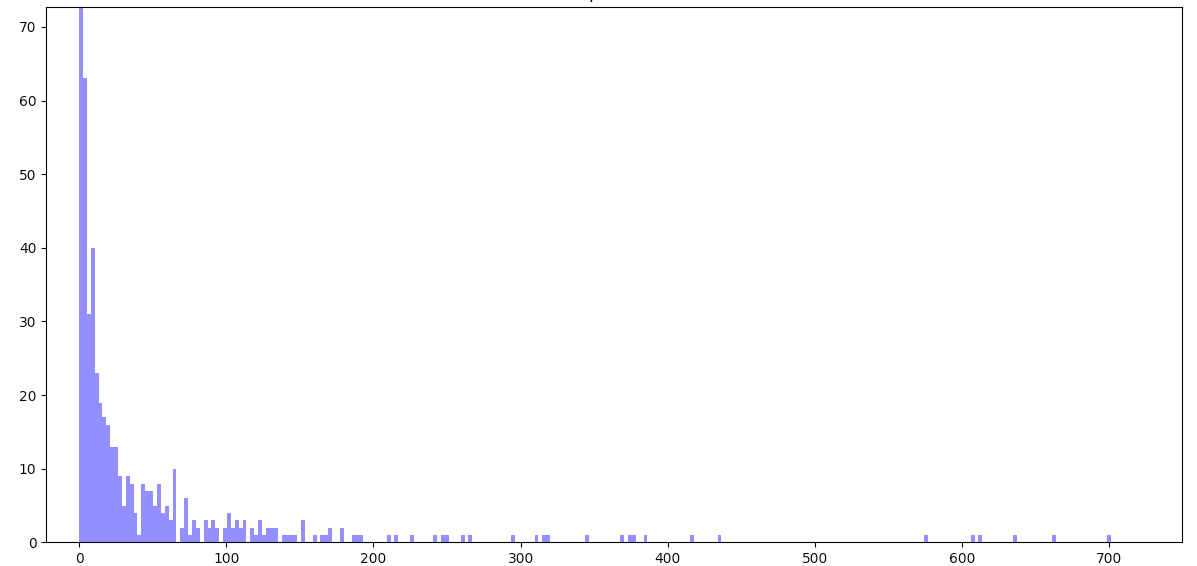
\includegraphics[width=\linewidth]{num_proteins_fold_155}
	\caption{Frequency of classes}
	\label{fig:boat1}
\end{figure}

We inspect the distribution of the proteins across the different folds. We see that most of the folds do not have a lot of proteins. The median number of proteins per fold was 10 and the histogram [Ref: Figure] show that most of our proteins have less than 50 proteins per fold. This would likely impact our learning, since there are not too many examples for the protein to learn.

We split up 70\% of the dataset for training, 15\% for validation and 15\% for testing. We adjust the sampling of the validation and testing so that a wide range of folds are represented.

New methods were tested on the small dataset. This allowed us to quickly prototype and optimize our methods to run on the larger dataset.

\subsubsection{Large Dataset SCOPe2.07}

SCOPe 2.07 is a database of 276,231 proteins that have been organized into 7 Classes, 1232 Folds, 2026 Superfamilies, and 4919 Families. The dataset was released and updated till 2017. This dataset contains and is about 9 times larger than the SCOP 1.55 dataset.

[Fig: Freq of data across folds]

We inspect the distribution of the proteins across the different folds. We see that there are much more proteins per fold.

Similar to the small dataset, we split up 70\% of the dataset for training, 15\% for validation and 15\% for testing. We adjust the sampling of the validation and testing so that a wide range of folds are represented.
	
\subsection{Third Party Tools}

A number of third party tools were used as part of the research. ProDy's (Protein Dynamics \& Sequence Analysis) python package was used to extract the backbone structure from each protein's PDB file. NumPy package was used for matrix  and statistical operations. Matplotlib package was used to generate histograms and 3D plots of the proteins and the barcodes. Pillow was used to generate the 2D images of the distance matrix and the barcode images. Keras and Tensorflow were used to setup and train the convolutional neural network. CPickle package was used to serialize and deserialize processed data.
	
\subsection{Computing Resources}

Initially the research started on a personal laptop without a GPU and very limited storage space [Ref: Table]. Since the unpacked data of SCOPe 2.07 took up around 40GB and the laptop ran out of storage space, the data was stored on a flash drive. 

The lack of a GPU made the training very slow. Even relatively simple methods on the smaller, SCOP 1.55, dataset took around 40 hours. Furthermore, the small storage space made it difficult to unpack and save the processed data on the larger SCOPe 2.07 dataset. These factors significantly slowed the progress of the research.


\begin{table}[t]
	\centering
	\begin{tabular}{c | c}
		CPU & Intel Core i7-4650U \\ \hline
		GPU (CUDA-enabled) & None     \\ \hline
		RAM & 8GB    \\ \hline
		Storage & 128GB SSD \\ \hline
		OS & MacOSx  
	\end{tabular}
	\caption{Personal Latop}
	\label{tbl:Computer 1}
\end{table}

Due to the limitations of the personal laptop, a personal workstation was purchased at \$500 on Winter of 2018 [Ref: Table]. Although it has modest computing power relative to industry standards, the purchased machine led to significant increases in speed and efficiency of the research. The most important changes in computer resources were the GPU, which led to increases in training speed, and the increased storage, which made it possible to work on the larger SCOPe 2.07 dataset. It is also worth nothing that Ubuntu has better support than MacOSx for running CUDA.
Most of the optimized methods took around 16 hours at most to complete on the large SCOPe 2.07 database, which is 8 times larger than the smaller SCOP 1.55. 

\begin{table}[t]
	\centering
	\begin{tabular}{c | c}
		CPU & E5-2630 6-Core \\ \hline
		GPU (CUDA-enabled) & Nvidia GTX 1060 6GB     \\ \hline
		RAM & 16GB    \\ \hline
		Storage & 500GB SSD \\ \hline
		OS & Ubuntu 16.02  
	\end{tabular}
	\caption{Personal Workstation}
	\label{tbl:Computer 2}
\end{table}

% ===============================================================
\section{Methods}
% ===============================================================

%---------------------
\subsection{ Background Information: Proteins}
%---------------------
A protein is an sequence of amino acids, 22 compounds which link into a protein chain. The interaction between amino acids and the surrounding environment determine the how the protein folds into its structure.

For a protein that we are tasked to classify, we are provided with many information: Protein sequence and the sequential coordinates of every atom on our protein. Since we are primarily interested in the topological features of our data, we characterize the protein's shape with the protein backbone. The protein's backbone is constructed with a sequence of points, where each point represents each amino acid in a 3D space. The point representation of each amino acid is determined by the algorithm 'parsePDB' in the ProDy package. 

Since we will be dealing primarily with the protein's backbone, we introduce the following notation.
	
\begin{defn}
A protein, `$P$`, with sequence of N amino acids will be a called a protein with length N. It's backbone will be denoted as a sequence of 3D coordinate points `$ \{P_i\}^{N}_{i=1} $` where `$P_{i} \in \mathbb{R}^3 $`

For each coordinate point `$ P_{i} $`, the x-coordinate is referred as `$ P_{i}(1) $`, y-coordinate as `$ P_{i}(2) $`, and z-coordinate as `$ P_{i}(3) $`.
\end{defn}

We extract two distinguishing types of input features from the protein's backbone chain: Distance matrix and Persistence Homology. These two features are very robust. They are both rotation and translation invariant, meaning that the features remain the same even if the protein is rotated or moved. They are also very stable: minor changes to the data does not create a significant variation in the feature.
	
%---------------------
\subsection{ Backbone Chain}
%---------------------	
Each the dataset of proteins are stored as PDB (Protein Data Bank) files, which describe the shape of the 3D protein. The dataset tar [Ref] files unpack into main directory, pdbstyle-1.55 and pdbstyle-2.07 for SCOP 1.55 and SCOPe 2.07 respectively. Each PDB file is stored in a subdirectory under the main directory. The name of the subdirectory is determined by the protein's name.

The index files for SCOP 1.55 and SCOPe 2.07, 'dir.cla.scop.1.55.txt' and 'dir.cla.scope.2.07-stable.txt', provide important information for each protein in our database [Ref: index example]. 

\begin{table}[t]
	\centering
	\begin{tabular}{c | c}
		Index Line & d1dlwa\_ 1dlw    A:  a.1.1.1 ... \\
		Name & d1dlwa\_     \\
		Class.Folds.Superfamily.Family & a.1.1.1    \\
	\end{tabular}
	\caption{Index Entry. The PDB file for this protein found under the subdirectory 'dl' as 'd1dlwa\_.ent'}
	\label{tbl:Index Entry}
\end{table}

For each protein, protein backbone chain is parsed from the PDB file using the 'parsePDB' function in the ProDy package. The extracted coordinates of the protein backbone is saved as a list. 

The class and the fold number of the protein uniquely identifies a protein's fold. We create a one to one mapping between class-fold to the integers. These integers are the labels of our protein-fold classification problem.

Because all of the protein coordinates do not fit on the RAM, they are saved in batches of 10000. In each batch, the protein coordinates and the fold labels are saved into a dictionary under the keys b'x' and b'y' respectively.

%---------------------
\subsection{ Distance Matrix}
%---------------------
With the points in the protein backbone, we construct a distance matrix of the distances between the points. The unit of the distances Ångströms, the units of provided in the protein PDB files. [Protein Data Bank]. We used the Euclidean Distance for the distances between the points.

	
\begin{defn}
	For a protein $P$ with length N, we denote it's distance as matrix $M_{P}$.
	We construct it as follows.
	$ M_{P} := [M_{ij}] $ where 
	\begin{multline*}
	M_{ij} = Euclidean Distance(P_i, P_j) = \\ \sqrt{P_i(1)-P_j(1))^2+(P_i(2)-P_j(2))^2} \\ +(P_i(3)-P_j(3))^2
	\end{multline*}
\end{defn}

\noindent
\textbf{Remark}
\\
	We note the following for any distance matrix $M_{P}$.
	\begin{itemize}
		\item $M_{ii} = 0$
		\item $M_{ij} = M_{ji}$
		\item The intersection of the ith row and the jth column corresponds to $M_{ij}$, the distance between the ith and the jth point.
	\end{itemize}
	
\begin{figure}[h]
	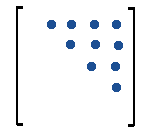
\includegraphics[width=\linewidth]{uptry.png}
	\caption{}
	\label{fig:uptry}
\end{figure}
	

We see that the distance matrix is symmetric [Ref: Remark] since the distance between the ith and the jth point is the same as the distance between the jth point and the ith point. Because of this, we only need to compute the distance between these pairs of points once. Also, the distance between a point to itself is zero. So the pairs of ith and jth's points we need to compute the distances for lie in the upper triangular region of the distance matrix. This region is consists of $\{ M_{ij} \space | \space i<j \}$ [Ref:]. Computing the distance matrix in this fashion divides the computation time by about half. Because the distance matrices of the entire dataset are larger than the size of the RAM, the data is split up into 1000 sized batches. 



\begin{figure}[h]
	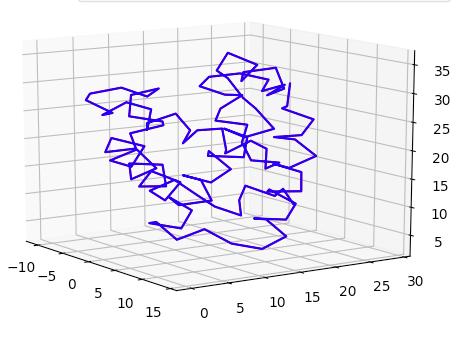
\includegraphics[width=\linewidth]{1ux8pdb.png}
	\caption{}
	\label{fig:network}
\end{figure}

We inspect the topological structure of our protein '1ux8'. It is a protein of length 118. This protein has some spiral structures (alpha helix). These spiral structures sometimes lie in close promixity in parallel or anti parallel direction (beta sheet). These types of structures (secondar structures) are known in molecular biology to be important features of a protein's shape.

\begin{figure}[h]
	\centering
	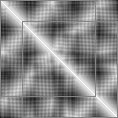
\includegraphics[width=.7\linewidth]{1ux8matBase}
	\caption{}
	\label{fig:network}
\end{figure}
	
We analyze the distance matrix to see if important structural features are represented in the matrix. To help with visualization, the distance matrix is mapped to an image of equal size, where closest distances appear in white and furthest distances appear in black. Distances in between take a gray hue with the intensity based on its value.
\\
\textbf{Feature Protein Backbone:}
Along the diagonal line of the image, the distance matrix is completely white. This is because the distance between a point to itself is zero [Ref: Remark]. We note that this diagonal white line uniquely identifies the protein backbone chain (Since the distance between. Having a clear representation of the protein backbone is important because  it is a central structure that other features can be spatially oriented around.
\noindent
\textbf{Feature Alpha Helix:}
We note thick white regions running parallel along the diagonal line of the image [Ref: Image]. These regions indicate that at a given point in the chain, it is in close proximity to the nearby neighbors [Ref Diagram]. We also note that in for a point in an Alpha Helix, it is also in close proximity to it's nearby neighbors. In our example, these four thick white regions correspond the the four helix structures on our protein.
	
\begin{figure}[h]
	\centering
	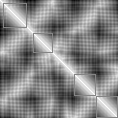
\includegraphics[width=.7\linewidth]{1ux8matAhelix}
	\caption{}
	\label{fig:network}
\end{figure}

	
\begin{figure}[h]
	\centering
	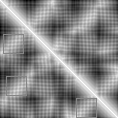
\includegraphics[width=.7\linewidth]{1ux8matBetaSheets}
	\caption{}
	\label{fig:network}
\end{figure}

\begin{defn}
A helix is composed of points in the protein backbone. Suppose $H$ is the set of indices of these points along the length of the protein. We call the row belonging to this helix as the collection of rows, $R_{i}$, of the distance matrix such that the rows contain elements of the helix. $\{R_{i} \space | \space i \in H \}$. Similarly we define the column belonging to the helix as $\{C_{i} \space | \space i \in H \}$.
\end{defn}

\noindent
\textbf{Feature Beta Sheet:}
We note patches of thick white regions in the intersection of the rows belonging to a helix and the columns belonging to another helix [Ref Diagram]. This indicates that the points of the two helices, and hence the two helices, are in close proximity. In particular, the regions are close sequentially: the ith point in helix A is close to the jth point in helix B and the i+1 th point in helix A is close to the j-1 th point in helix B. This sequential relationship describes a Anti-parallel Beta Sheets. For Parallel Beta Sheets, the i+1 th point would be close to the j+1 th point. In our example, the 3 pairs of Beta-sheets formed the 4 helices are represented in our distance matrix.
	
\subsubsection{ Cropped Distance Matrix}

Some proteins have a length of 600, making the distance matrix have a size of 600x600. However, due limitations on the GPU memory, it is not possible to construct a convolutional network with our input being 600x600. We would also like to crop the distance matrix such that the central backbone of the protein runs through the diagonal of our matrix. To crop and preserve the diagonal protein backbone, we take a 100x100 window and crop our matrix by shifting row and columns at the same time by 50 indices.

\begin{figure}[h]
	\centering
	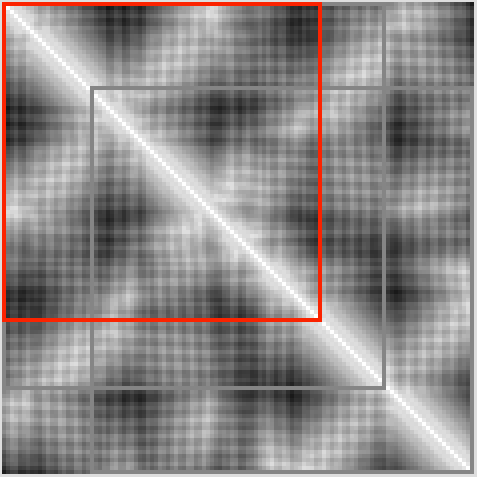
\includegraphics[width=.7\linewidth]{cropMat}
	\caption{}
	\label{fig:network}
\end{figure}

Because of the limitations set by the windowed distance matrix, a point in the backbone can only see information about, on average, half of the window size forwards and backwards. This limitation affects the cropped matrix's ability to detect longer range contact information, which can be critical in determining the protein's overall shape. In our example [Ref], the cropped distance matrix would not see information about the proximity between the first alpha helix and the third alpha helix because they are too far away in the backbone index.

\begin{figure}[h]
	\centering
	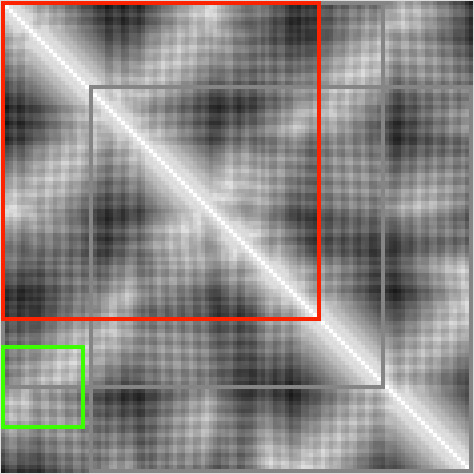
\includegraphics[width=\linewidth]{cropMatMiss}
	\caption{}
	\label{fig:network}
\end{figure}

Cropping the dataset increases the number of examples in the dataset. Because we don't want our training data to have similarities, we make sure that the training, validation, and testing groups do not share cropped matrices from the same protein.

\subsubsection{ Sparse Distance Matrix}

In our example, we see that cropping the distance matrix diminishes it's ability to represent long range contact information. We develop an alternative approach to reduce the size of the distance matrix while preserving it's ability to represent long range contact information.

\begin{figure}[h]
	\centering
	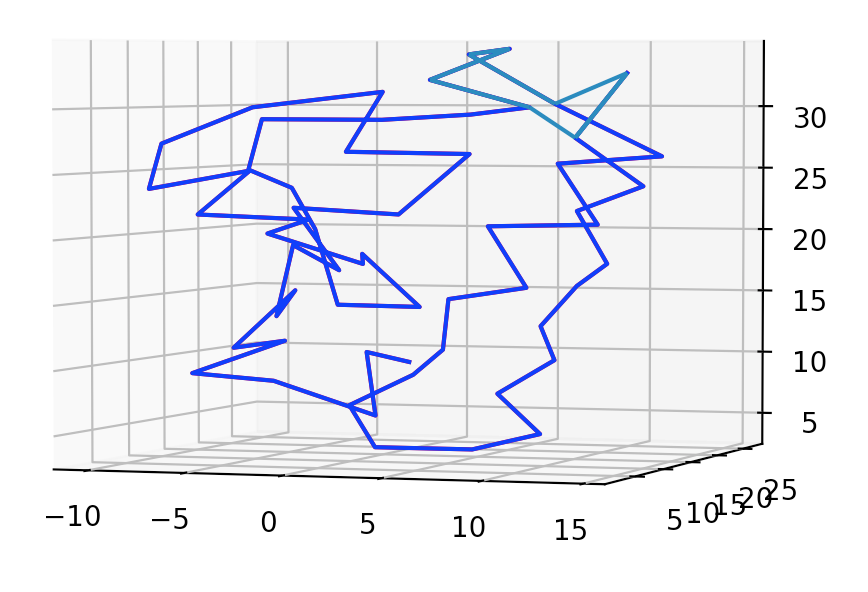
\includegraphics[width=\linewidth]{1ux8sparse}
	\caption{}
	\label{fig:network}
\end{figure}

Given, a protein backbone with length N, $\{P_i\}^{N}_{i=1}$, we sample every other point, $\{P_i \space | \space \text{i is odd} \}$, to create a sparse protein backbone. We graph the sparse protein backbone in 3D space [Ref ] and compare it to the original protein backbone [Ref: Original Chain]. In comparison, we see that the general structure of the protein and its features are diminished but preserved.

\begin{figure}[h]
	\centering
	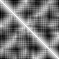
\includegraphics[width=.7\linewidth]{1ux8pdbSparseDistM}
	\caption{}
	\label{fig:network}
\end{figure}

From the sparse protein backbone, we construct a sparse distance matrix in the same fashion as a regular distance matrix. In example, we compare the sparse distance matrix [Ref:] and the unmodified distance matrix [Ref:] and see if the backbone chain, alpha helix and beta sheet features are preserved in the distance matrix. First, we see that the diagonal backbone is preserved in the matrix. Second, we do see that the alpha helix features are preserved, even though it is less clearly defined. Finally, we see that the beta sheet features are preserved as well.

For the protein of length 600, the sparse distance matrix would reduce the matrix's size from 600x600 to 300x300. This is still too big for due to the limitations on the GPU memory. So we crop the sparse distance matrix in the same manner as a regular distance matrix. We also take care such that the training, validation, and testing groups do not share cropped matrices from the same protein.

%----------------------
\subsection{Convolutional Network Model}
%----------------------

The features from each of these subsections were fed into a a 2D-convolutional network. The architecture of the 2D-convolutional network for mapping protein structure to folds contains, in order, 32 3x3 convolutional layers, 64 3x3 convolutional layers, 2x2 max pooling, 128 dense layer, and the output layer.

\begin{figure}[h]
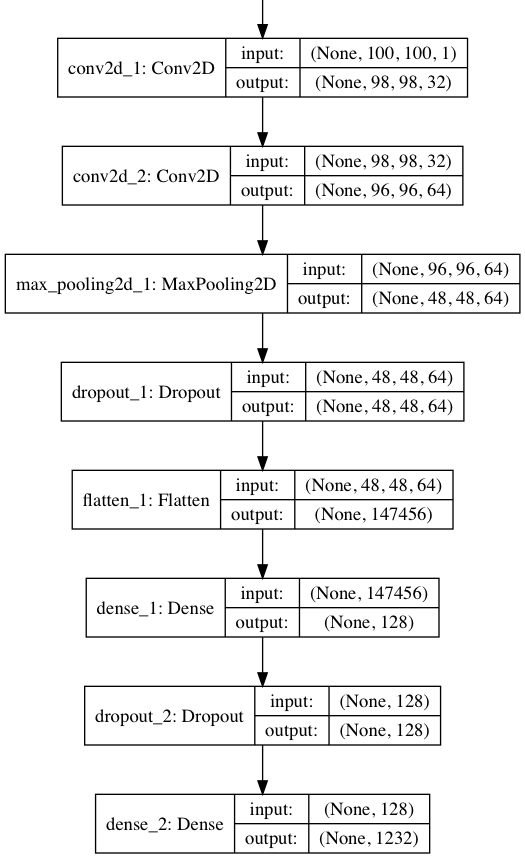
\includegraphics[width=\linewidth]{model_plot.png}
\caption{The architecture of a 2D deep convolutional network for fold classification.}
\label{fig:network}
\end{figure}

This is a relatively simple network. However, for our task of classifying quarter million of proteins, it performs exceptionally well. 
\\
There are a lot of benefits for a simple network performing well. First, it ensures that the model is not overfitting the data. Second, it is much more feasible to inspect the network to understand how it is learning.


%---------------------
\subsection{ Topological Data Analysis}
%---------------------
\textbf{Persistent Homology: } Topological data analysis is applied to the points in the protein backbone to produce persistent barcodes. The barcodes indicate when simplexes are formed and are destroyed. Significant topological features of the data are represented by these barcodes.


\begin{figure}[h]
	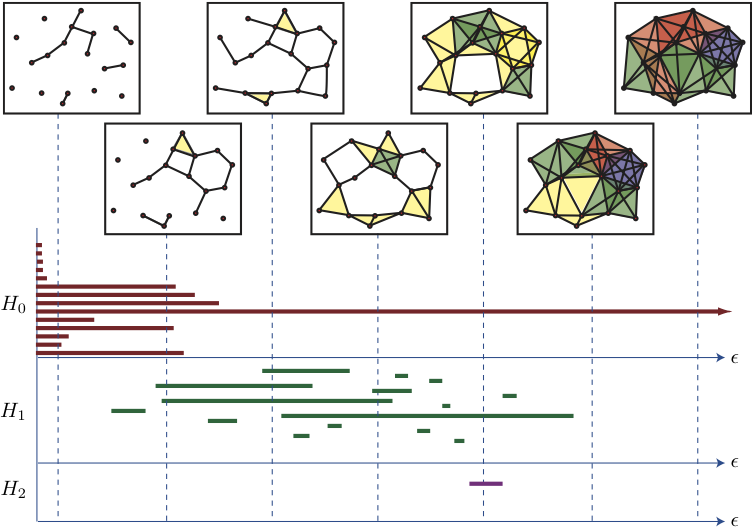
\includegraphics[width=\linewidth]{tdaexample.png}
	\caption{Topological data analysis on a set point cloud}
	\label{fig:tdaex}
\end{figure}


\subsubsection{ Mathematical Background}

\subsubsection{Persistence Homology}
As a visualization, we run the TDA on 2b7h, a protein of length ~120. We see that the barcodes do represent significant features of the protein such as alpha helices and beta sheets.

\begin{figure}[t]
	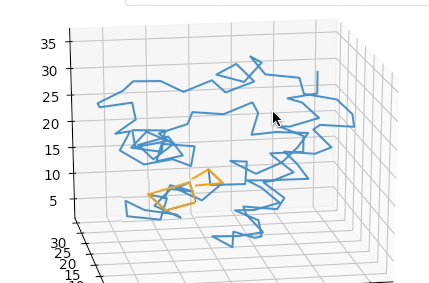
\includegraphics[width=\linewidth]{helixsimplex.png}
	\caption{TDA 2b7h detecting alpha helices }
	\label{fig:tdahelix}
\end{figure}

\begin{figure}[t]
	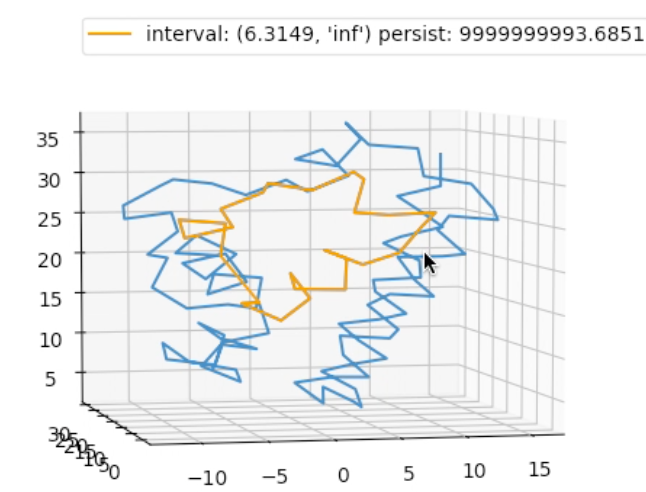
\includegraphics[width=\linewidth]{betasimplex.png}
	\caption{TDA 2b7h detecting beta sheets }
	\label{fig:tdabeta}
\end{figure}


\begin{figure}
	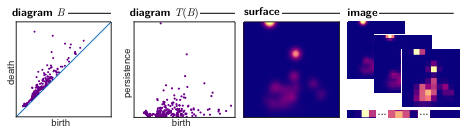
\includegraphics[width=\linewidth]{persistenceimages.png}
	\caption{Persistence Images}
	\label{fig:boat1}
\end{figure}
\subsubsection{ Sparse Persistence Homology}
\subsubsection{ Backbone Aware Persistence Homology}
\subsubsection{ Persistence Images}
We format the barcode data into three separate input features: persistent images, simplex distance map, and simplex grouping
\\
\textbf{Persistent Images:} The barcodes for each simplex are mapped into a 2-dimensional vector space with the first coordinate being the birth and the second coordinate being the persistence of the simplex. The plot cropped and converted to a blurred image at a set resolution. The range of the first and second coordinates to crop the plot were derived from the distribution of the data.

\begin{figure}
	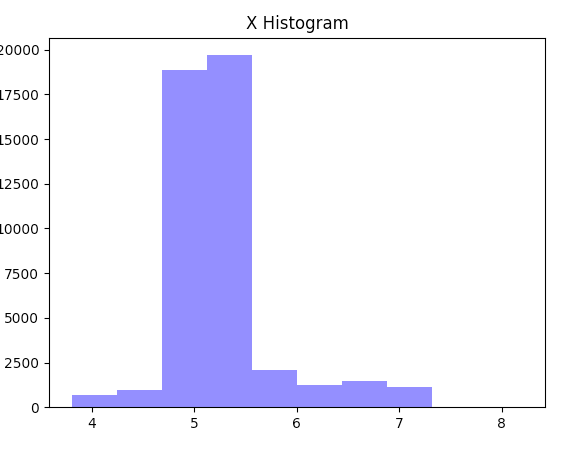
\includegraphics[width=\linewidth]{xhist.png}
	\caption{x range}
	\label{fig:boat1}
\end{figure}

\begin{figure}
	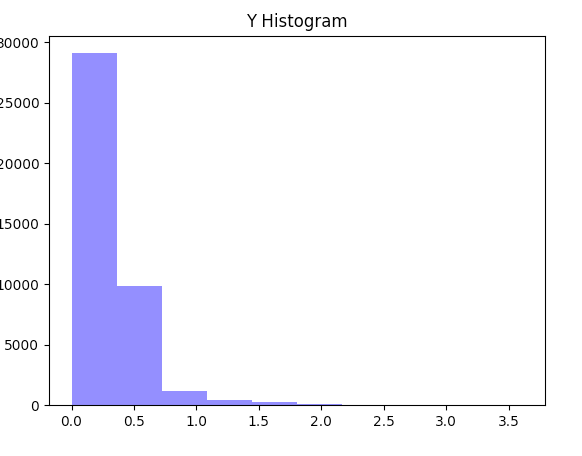
\includegraphics[width=\linewidth]{yhist.png}
	\caption{y range}
	\label{fig:boat1}
\end{figure}


% ===============================================================
\section{Results}
% ===============================================================

%----------------------
\subsection{Distance Matrix Algorithm}
%----------------------
	The distance matrix as the input feature worked pretty well for classifying the data. The best method, subsampling every other point with a window size of 50x50 gives an accuracy of 96\%
	
	The other two methods perform pretty well, at around 86\%.
	The subsampling method probably works best because it gives the neural network model to view the long range dependencies.
	The smaller window size of 50x50 performs much better than the 100x100 window for the subsampling methods.	
	
	\begin{figure}[t]
	  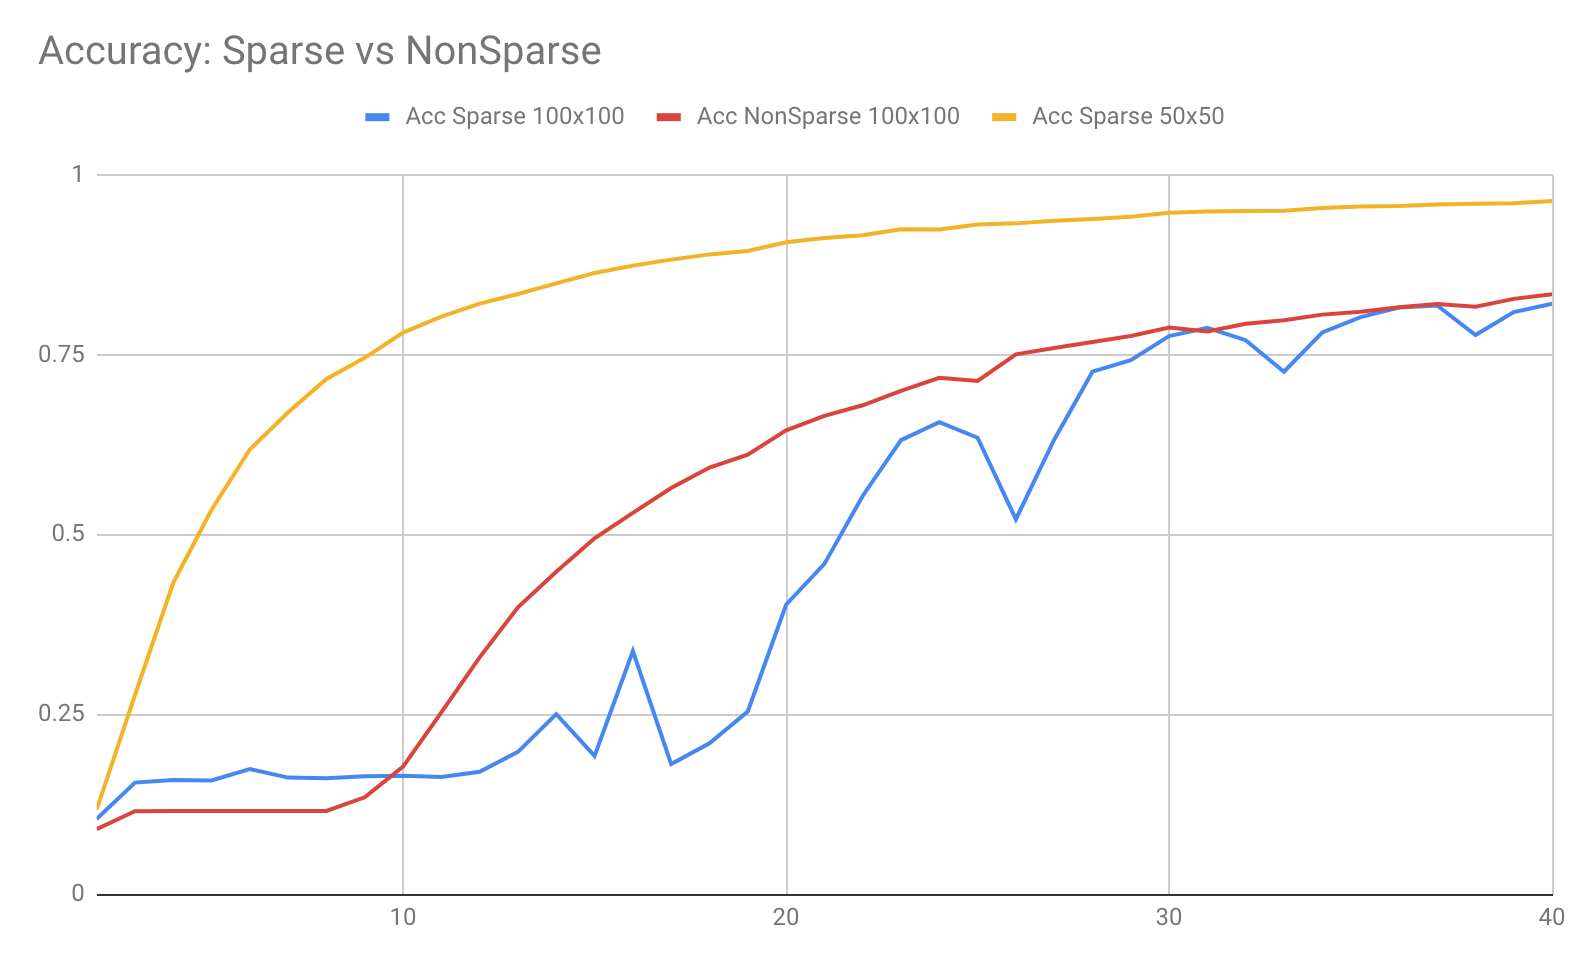
\includegraphics[width=\linewidth]{AccSparsevsNonSparse.png}
	  \caption{}
	  \label{fig:network}
	\end{figure}
	
	\begin{figure}[t]
	  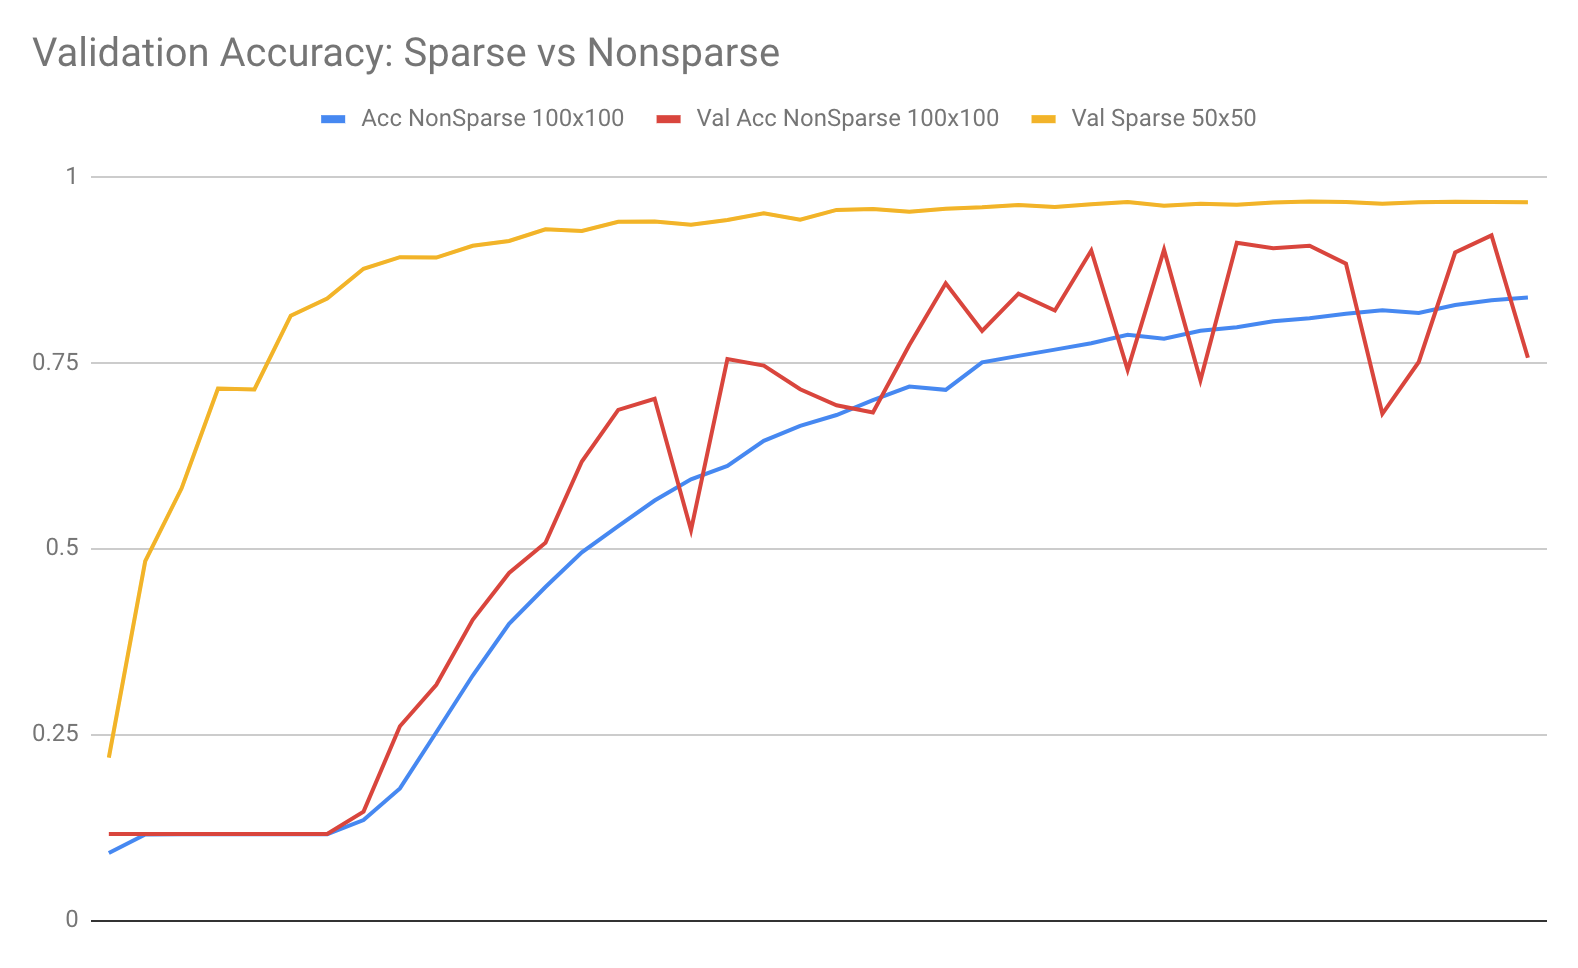
\includegraphics[width=\linewidth]{ValAccSparsevsNonsparse.png}
	  \caption{}
	  \label{fig:network}
	\end{figure}


%------------------------------------------------
%
%\section{Table, Figure, List Examples}
%
%\begin{figure}
%  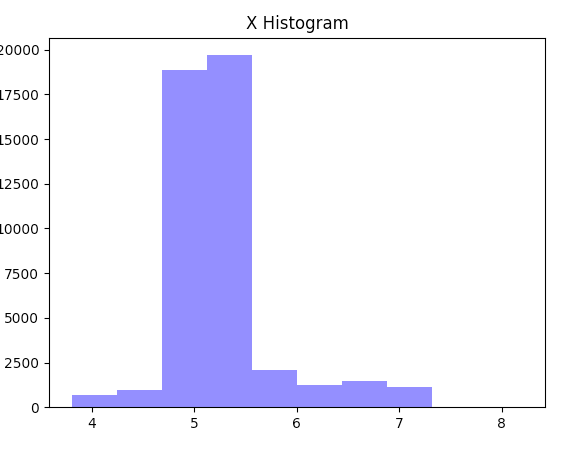
\includegraphics[width=\linewidth]{xhist.png}
%  \caption{A boat.}
%  \label{fig:boat1}
%\end{figure}
%
%\begin{table}[]
%\begin{tabular}{ccc}
%\hline
% a & a & a \\ \hline
% a & a & a \\
% a & a & a \\
% a & a & a
%\end{tabular}
%\end{table}
%
%
%\begin{itemize}
%	\item First item in a list 
%	\item Second item in a list 
%	\item Third item in a list
%\end{itemize}
%
%\begin{description}
%	\item[First] This is the first item
%	\item[Last] This is the last item
%\end{description}
%
%\begin{enumerate}
%	\item First numbered item in a list
%	\item Second numbered item in a list
%	\item Third numbered item in a list
%\end{enumerate}


%-------------------------------
%	BIBLIOGRAPHY
%---------------------------------
\pagebreak
 
\begin{thebibliography}{9}

\bibitem{persistenceImages} 
Henry Adams, Tegan Emerson, and Michael Kirby. 
2017.
\textit{Persistence Images: A Stable Vector Representation of
Persistent Homology}. 
Journal of Machine Learning Research 18 (2017) 1-35

\bibitem{deepsf}
Jie Hou, Badri Adhikari and Jianlin Cheng.
2018.
\textit{DeepSF: deep convolutional neural network for mapping protein sequences to folds}
Bioinformatics, 34(8), 2018, 1295–1303

\bibitem{sakai}
Katsuro Sakai.
2010.
\textit{Simplicial Homology — A Short Course}
Institute of Mathematics University of Tsukuba

\bibitem{scope}
Fox NK, Brenner SE, Chandonia JM.
2014.
\textit{SCOPe: Structural Classification of Proteins—extended, integrating SCOP and ASTRAL data and classification of new structures.}
Nucleic Acids Research 42:D304-309. doi: 10.1093/nar/gkt1240


\bibitem{pdb}
Protein Data Bank Guide
\textit{Protein Data Bank Changes Guide
	New Changes in Version 3.20}
Nucleic Acids Research 42:D304-309. doi: 10.1093/nar/gkt1240
https://cdn.rcsb.org/wwpdb/docs/documentation/file-format/changesv3.20.pdf

\end{thebibliography}

\end{document}
